\chapter{Variaciones del Modelo}\label{chap:variaciones}

Teniendo ya claros los conceptos médicos y el análisis de un modelo base acorde con tales conceptos, es momento de introducir al modelo las dos enfermedades presentadas en la sección \ref{sec:RBC:enfermedades}: el caso de las hemorragias y el de la anemia. Los sangrados son tratados una única vez (hasta que sean frenados), mientras que la anemia es una enfermedad cuyo tratamiento es para toda la vida. En este capítulo se presentarán las variaciones matemáticas del modelo y el análisis de las simulaciones de estas variaciones, esperando que los resultados obtenidos logren mantener la homeostasis del paciente y, para el caso de la anemia, ver si un aumento o disminución de la dosis afecta realmente los resultados.

\section{Caso con Hemorragia}\label{Sec:variaciones:hemorragia}

Para los sangrados, se tendrán en cuenta diferentes casos. Inicialmente se tendrá en cuenta una hemorragia leve (pérdida del 2$\%$ de sangre) y se observará lo que sucede si, después de la pérdida de sangre, las variables del modelo se mantienen iguales y que sucede si estas se modifican. Posteriormente se considerará el caso de una hemorragia grave (el 14$\%$ de la sangre del cuerpo, que Holland lo considera grave pero no fatal en \cite{PerdidaSangre}) y se observarán los efectos de una transfusión sanguínea para recuperar la homeostasis. En el caso de las hemorragias, se tendrá en cuenta el caso en el que $\gamma =1$, pues así el paciente es totalmente sano, el parámetro $f$ se mantiene igual que antes ($=0.00832$) y los valores iniciales también se mantienen.

\subsection{Hemorragia Leve}\label{subsec:variaciones:hemorragia:leve}

Para esta variación del modelo, tome como ejemplo que en el tercer día de medición el paciente, ya sea por un corte o un accidente, pierde el $2\%$ de su cantidad de sangre en el cuerpo que, considerando el caso de que tenga 5 litros de sangre, esto equivale a 100 mililitros de fluido o a $5\times 10^{11}$ glóbulos rojos. Así, el modelo se puede ver de la siguiente manera:

\begin{align}\label{eq:HemoLeveMal}
    R(n+1) &= \left\{ \begin{array}{lcc} (1-f)\cdot R(n)+M(n) & \textrm{si} & n \neq 3 \\ \\ (1-f)\cdot R(n)+M(n)-0.02\cdot R(n) & \textrm{si} & n = 3\end{array} \right., \\
    M(n+1) &=\gamma \cdot f \cdot R(n). \nonumber
\end{align}

En donde:
\begin{itemize}
    \item $\gamma=1$; (glóbulos rojos producidos por cada uno perdido)
    \item $f=0.00832$; (fracción de glóbulos rojos eliminados diariamente)
    \item $R(0) = 25\times 10^{12}$; (cantidad inicial de glóbulos rojos)
    \item $M(0) = 208 \times 10^{9}$. (RBC's eliminados por la médula ósea en el día 0)
\end{itemize}

La simulación se ve así: en la primera gráfica de la figura \ref{sec:variaciones:fig:HemoLeveG1} se observa la pérdida de RBC's en el tercer día, un aumento en la cantidad de eritrocitos del tercero al cuarto y estabilidad del cuarto en adelante. En la segunda gráfica se observa lo mismo pero con un día de atraso. El aumento de RBC's que se puede observar está dado por el hecho de que el adendo $M(n)$ conserva lo que ha ocurrido en $R(n-1)$ así, para el cuarto día se producen la cantidad de eritrocitos que se vienen produciendo regularmente antes del accidente, y desde el cuarto día en adelante este adendo ya se acomoda a la nueva cantidad de sangre. La estabilidad en los glóbulos rojos que se observa del cuarto día en adelante está dada por el hecho de que $\gamma = 1$. El modelo, de esta manera, funciona como lo hace normalmente (véase la sección \ref{subsec:modelo:simulaciones:G1}) tomando una cantidad inicial de sangre menor que la original, es decir que mantiene una estabilidad con la cantidad de RBC's del cuarto día, que es de $24.504\times 10^{12}$ glóbulos rojos. 

\begin{figure}[H]
    \centering
    \captionsetup{justification=centering}
    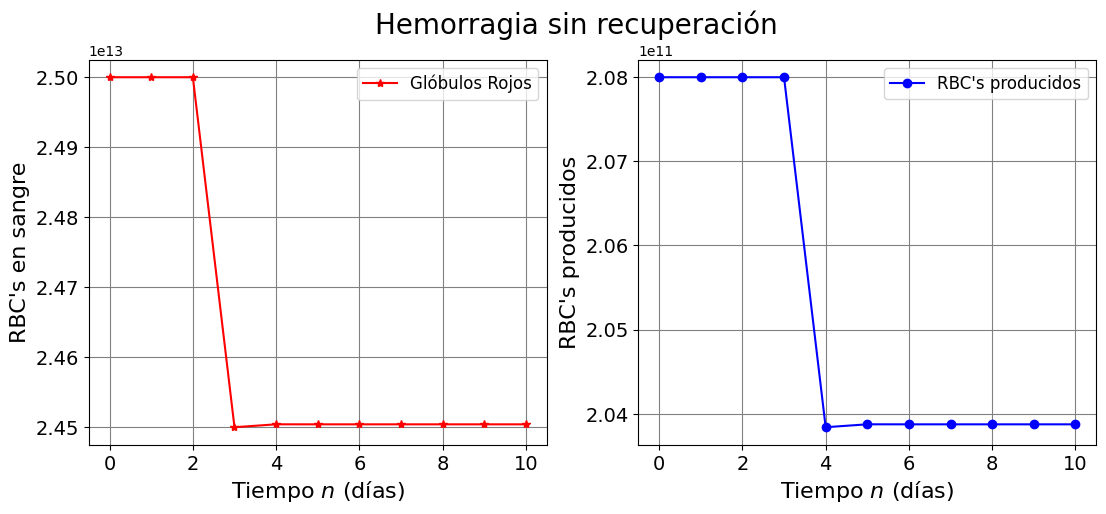
\includegraphics[scale=0.534]{figures/HemoLeveG1.png}
    \caption{Simulación del modelo para el caso de una hemorragia sin recuperación de la homeostasis. A la izquierda está la gráfica de $R(n)$, a la derecha la de $M(n)$.}
    \label{sec:variaciones:fig:HemoLeveG1}
\end{figure}

Está claro que esta simulación está totalmente alejada de lo que ocurre en el caso real, pues lo esperado es que el cuerpo recupere con el paso del tiempo la cantidad de glóbulos rojos perdidos, esto quiere decir que para $n>3$ se debe aumentar el valor de $\gamma$ hasta que la cantidad de eritrocitos sea mayor o igual a la inicial, es decir:

\begin{align}\label{eq:HemoLeveBien}
    R(n+1) &= \left\{ \begin{array}{lcc} (1-f)\cdot R(n)+M(n) & \textrm{si} & n \neq 3 \\ \\ (1-f)\cdot R(n)+M(n)-0.02\cdot R(n) & \textrm{si} & n = 3\end{array} \right. \\
    M(n+1) &=\left\{ \begin{array}{lcc} f\cdot \gamma_1 \cdot R(n) & \textrm{si} & R(n+1) \geq R(0) \\ \\ f\cdot \gamma_2\cdot R(n) & \textrm{si} & R(n+1)<R(0)\end{array} \right. \nonumber
\end{align}

La condición de $M(n+1)$ permite evitar el retraso del que se ha hablado anteriormente, pues si se considera que ya se alcanzó la cantidad ``normal'' de eritrocitos entonces el cuerpo no debe producir más de los necesarios.

Para calibrar el valor de $\gamma_2$ se utilizó la información brindada por el hospital general de Massachusetts en \cite{Massachusetts}, dado que al cuerpo le toma recuperar los glóbulos rojos perdidos en 450 ml de sangre en unas 5 semanas (35 días), entonces 100 ml deben recuperarse en unos 8 días. Las simulaciones hechas muestran que $\gamma=1.305$ permite lograr esta recuperación en ese tiempo.

Así, los valores constantes a tener en cuenta son:
\begin{itemize}
    \item $\gamma_1=1$; (glóbulos rojos producidos por cada uno perdido normalmente)
    \item $\gamma_2=1.305$; (glóbulos rojos producidos por cada uno perdido después de la hemorragia)
    \item $f=0.00832$; (fracción de glóbulos rojos eliminados diariamente)
    \item $R(0) = 25\times 10^{12}$; (cantidad inicial de glóbulos rojos)
    \item $M(0) = 208 \times 10^{9}$. (RBC's eliminados por la médula ósea en el día 0)
\end{itemize}

Para estas simulaciones, se utilizó un tiempo de 15 días para poder observar lo que sucede después de recuperar los eritrocitos perdidos:

\begin{figure}[H]
    \centering
    \captionsetup{justification=centering}
    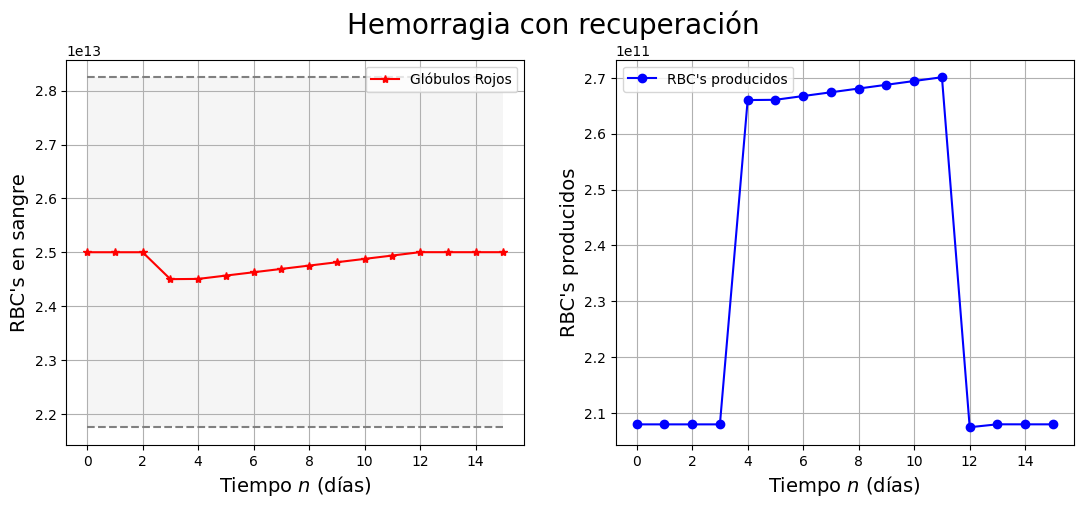
\includegraphics[scale=0.534]{figures/HemoLeveG13.png}
    \caption{Simulación del modelo para el caso de una hemorragia con recuperación de la homeostasis. A la izquierda está la gráfica de $R(n)$, a la derecha la de $M(n)$.}
    \label{sec:variaciones:fig:HemoLeveG13}
\end{figure}

Lo que se puede ver en estas gráficas es como, a partir del cuarto día (dado el retraso que presenta el modelo) se hace efectivo el cambio de $\gamma_1$ a $\gamma_2$, que se evidencia por el aumento en la primera gráfica de la figura \ref{sec:variaciones:fig:HemoLeveG13} del cuarto al duodécimo día y en la segunda gráfica del cuarto al undécimo día. En el día 12 es en el que por fin se ha superado (o igualado) la cantidad inicial de glóbulos rojos en el cuerpo, el aumento desde la pérdida muestra lo ilustrado en la sección \ref{subsec:modelo:simulaciones:G13}, donde hay un aumento constante de eritrocitos. Después de recuperar la cantidad de sangre perdida, el cuerpo vuelve a estabilizar su sistema, pues ha llegado a la homeostasis. La diferencia en la segunda gráfica de los días 0 a 3 y de los días 13 a 15 se debe a que ha aumentado la cantidad estable de sangre, y para compensar la pérdida el cuerpo debe producir más células.

Teniendo esto en cuenta, ahora se debe analizar el caso en el que el paciente sufre de una hemorragia más grave y debe ser sometido a una transfusión sanguínea para que pueda recuperarse.

\subsection{Hemorragia Grave}\label{subsec:variaciones:hemorragia:grave}

Considérese el caso en el que el paciente analizado sufre, por ejemplo, una pérdida del 14$\%$ del volumen de sangre de su cuerpo (unos 700 mililitros o 3.25$\times 10^{12}$ eritrocitos) a causa de un accidente, ya sea una hemorragia interna causada por un golpe o una herida externa como un corte. Esta pérdida de sangre, según Holland en \cite{PerdidaSangre}, se puede considerar como grave pero no crítica (no tiene efectos secundarios mayores), por lo que este ejemplo debe ser tratado médicamente mediante una transfusión sanguínea y no afectará las dinámicas normales del cuerpo.

Dado que las bolsas de transfusión de glóbulos rojos tienen un volumen aproximado de 250 mililitros (\cite{Granada}), correspondiente al 5$\%$ de la concentración normal, unos 1.25$\times 10^{12}$ RBC's, entonces para subsanar la pérdida del 14$\%$ se tomará como ejemplo que le son suministradas al paciente dos bolsas de eritrocitos y el volumen restante podrá ser recuperado por el cuerpo.

Para poder adecuar el modelo al problema, se considerará que el sangrado inicia y termina en el tercer día y el suministro de sangre ocurre y finaliza en el cuarto. Para la presente investigación es útil definir este caso de tal manera para poder ilustrar correctamente las ecuaciones. Es importante notar que el cuerpo tendrá tres estados diferentes durante este caso: la estabilidad antes y después de la recuperación, el estado del día en el que se hace la transfusión y el estado de los días después de la transfusión. De esta manera, el cuerpo debe modificar su producción interna de RBC's en tres momentos, generando dos valores nuevos de $\gamma$ para cada cantidad de glóbulos rojos.

Así, una hemorragia grave se puede interpretar con la siguiente modificación del modelo base:

\begin{align}\label{eq:HemoGrave}
    R(n+1) &= \left\{ \begin{array}{lcc} (1-f)\cdot R(n)+M(n) & \textrm{si} & n \neq 3,4 \\ \\ (1-f)\cdot R(n)+M(n)-0.14\cdot R(n) & \textrm{si} & n = 3 \\ \\ (1-f)\cdot R(n)+M(n)+0.1\cdot R(0) & \textrm{si} & n = 4 \\ \end{array} \right. \\
    M(n+1) &=\left\{ \begin{array}{lcc} f\cdot \gamma_1 \cdot R(n) & \textrm{si} & R(n+1) \geq R(0) \\ \\ f\cdot \gamma_2\cdot R(n) & \textrm{si} & n = 4\textrm{ y } R(n+1)<R(0) \\ \\ f\cdot \gamma_3\cdot R(n) & \textrm{si} & n \neq 4\textrm{ y } R(n+1)<R(0)\\ \end{array} \right. \nonumber
\end{align}

Los valores de $\gamma_2$ y $\gamma_3$ fueron estimados al igual que en el caso de hemorragias leves. La cantidad de glóbulos rojos perdida en 700 mililitros de sangre debería ser recuperada por el cuerpo en unos 55 días, obteniendo un valor de $\gamma_2$ de 1.331. Para calibrar $\gamma_3$ se debe tener en cuenta la cantidad de eritrocitos en el cuerpo en el quinto día, pues el cuerpo del paciente se ajusta a la nueva cantidad de glóbulos rojos obtenidos gracias a la transfusión. En el quinto día de simulación, el cuerpo tiene 24.0673$\times 10^{12}$ RBC's, siguiendo la cuenta del hospital general de Massachusetts (\cite{Massachusetts}), la cantidad restante (93.2713 $\times 10^{10}$ eritrocitos) se recuperaría en 15 días, se concluye que $\gamma_3 = 1.31$ según las simulaciones del modelo.

Así, los valores constantes a tener en cuenta son:
\begin{itemize}
    \item $\gamma_1=1$; (glóbulos rojos producidos por cada uno perdido normalmente)
    \item $\gamma_2=1.305$; (glóbulos rojos producidos por cada uno perdido después de la hemorragia)
    \item $\gamma_3=1.31$; (glóbulos rojos producidos por cada uno perdido después de la transfusión)
    \item $f=0.00832$; (fracción de glóbulos rojos eliminados diariamente)
    \item $R(0) = 25\times 10^{12}$; (cantidad inicial de glóbulos rojos)
    \item $M(0) = 208 \times 10^{9}$. (RBC's eliminados por la médula ósea en el día 0)
\end{itemize}

Para ilustrar los diferentes estados del cuerpo mencionados anteriormente, se amplió el tiempo de simulación a 22 días: 

\begin{figure}[H]
    \centering
    \captionsetup{justification=centering}
    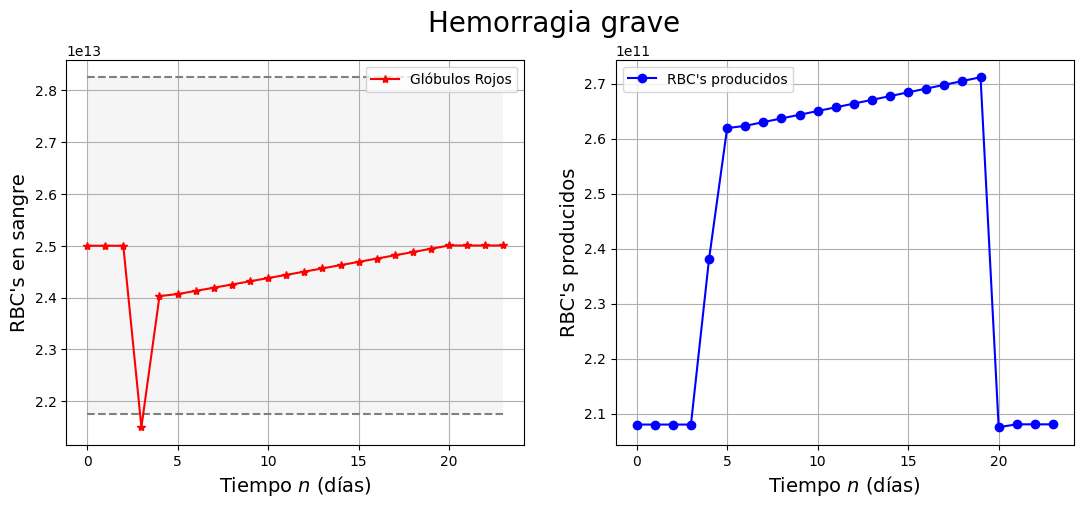
\includegraphics[scale=0.534]{figures/HemoGrave.png}
    \caption{Simulación del modelo para el caso de una hemorragia grave con transfusión. A la izquierda está la gráfica de $R(n)$, a la derecha la de $M(n)$.}
    \label{sec:variaciones:fig:HemoGrave}
\end{figure}

Para los primeros dos días, el cuerpo se encuentra en el estado estable de $\gamma = 1$. En el tercer día ocurre la hemorragia grave y se puede ver una amplia caída en la cantidad de glóbulos en la gráfica izquierda de la figura \ref{sec:variaciones:fig:HemoGrave}. Esta pérdida, sin embargo, se ve mitigada un poco debido a la producción normal de eritrocitos por parte de la médula ósea. A partir de este día inicia el fuerte crecimiento en la producción de RBC's, pues el cuerpo debe intentar recuperar lo perdido (gráfica derecha a partir del cuarto día). En el día cuatro se puede ver el efecto de la transfusión efectuada a través de un gran aumento en la cantidad de eritrocitos respecto al día anterior. En el quinto día hay en la gráfica izquierda una disminución en la pendiente respecto al día anterior que se debe a la transición de $\gamma_2$ a $\gamma_3$, y esto se ve reflejado en la primera gráfica por el cambio de pendiente en los días 4-5 y 5-6. A partir del quinto día el cuerpo produce glóbulos rojos según $\gamma_3$ hasta volver al valor inicial y así volver a la estabilidad brindada por $\gamma_1$.

Las gráficas permiten ilustrar la gran ventaja de la transfusión sanguínea, pues sin esta se recuperaría la sangre perdida en 55 días en vez de en 17.

\section{Caso con Anemia Renal}\label{Sec:variaciones:anemia}

Para este caso se considerará un paciente con anemia renal permanente producida por falta de eritropoyetina en el torrente sanguíneo, es decir que los riñones no segregan la suficiente cantidad de la hormona que le indica al cuerpo que debe acelerar la producción de RBC's. Este paciente debe ser tratado por el resto de su vida mediante la aplicación de eritropoyetina por vía intravenosa para poder elevar la producción de eritrocitos por parte de la médula ósea. 

La eritropoyetina, según el estudio del capítulo \ref{chap:RBC}, es la hormona encargada de fomentar la producción de glóbulos rojos por parte de la médula ósea. De esta manera, la cantidad de EPO en sangre debe afectar el resultado de $M(n)$ de alguna manera.

Para la investigación, se consideró que cada unidad por mililitro aplicada de EPO produce $10^{5}$ glóbulos rojos respecto a la producción de una persona sana. Esto quiere decir (en resumidas cuentas) que cada mU/ml de EPO aplicada aumenta un $0.01\%$ la producción de glóbulos rojos respecto a una persona sana. De esta manera, la ecuación de $M(n)$ se verá modificada de la siguiente manera: 

\begin{equation*}
    M(n+1)=\gamma\cdot f \cdot R(n)+\frac{\delta(n)*y_s}{10000},
\end{equation*}

es decir que la cantidad de glóbulos rojos producidos por la médula ósea en el día $n+1$ ahora también dependerá también de la cantidad que produzca la concentración de EPO en la sangre del paciente, $\delta(n)$, siguiendo la hipótesis mencionada anteriormente de la producción de $0.01\%$ por mU/ml aplicada respecto a la producción normal de un paciente sano, $y_s$. 

Esto implica que se debe definir una ecuación para $\delta(n)$. Esta se basa en el artículo de Frymoyer (\cite{FRYMOYER2019123}), en donde se puede modelar la concentración de una dosis de un fármaco aplicado por vía intravenosa ($\delta(t)$) mediante la ecuación diferencial

\begin{equation}\label{eq:diferencial}
    \dfrac{d\delta}{dt}=-k_e \delta(t),
\end{equation}

en donde $k_e$ es una constante que representa la velocidad a la que el cuerpo elimina el fármaco y es medida en 1/h. Para el caso de la eritropoyetina, Garzone en \cite{GARZONE2012547}, define $k_e=0.077$. La fracción $\dfrac{d\delta}{dt}$ está medida en [(mU/ml)/h], miliunidades por mililitro por hora, mientras que $\delta(t)$ está medido en mU/ml.

La solución de la ecuación diferencial \ref{eq:diferencial} es:

\begin{equation}\label{eq:solucionDif}
    \delta(t)=\delta_0\cdot e^{-k_e\cdot t},
\end{equation}

donde $\delta_0$ es la concentración de cada dosis.

Para poder modelar múltiples dosis de un fármaco, entonces se debe modificar la solución de la ecuación diferencial para que cuando se deba administrar la nueva dosis (aplicada cada $t_0$ horas), se considere la concentración de fármaco que queda en el cuerpo de la dosis anterior, esto se puede hacer de la siguiente manera:

considere $\delta_n$ como la concentración del fármaco en la sangre en la $n$-ésima dosis, entonce se tiene que 

\begin{align*}
    \delta_0 &= \delta_0,\\
    \delta_1 &= \delta_0 + \delta_0\cdot e^{-k_e\cdot t_0}, \\
    \delta_2 &= \delta_0 + \delta_1\cdot e^{-k_e\cdot t_0}= \delta_0\left(1+e^{-k_e\cdot t_0}+\left(e^{-k_e\cdot t_0}\right)^2\right), \\
    &\cdots \\
    \delta_n &= \delta_0(1+\alpha+\alpha^2+...+\alpha^{n}) \\
    \implies \delta_n &= \delta_0\left(\frac{1-\alpha^{n+1}}{1-\alpha}\right),\quad \alpha=e^{-k_e\cdot t_0}.
\end{align*}

Adecuando este resultado a la ecuación continua \ref{eq:solucionDif} se obtiene que, para cada intervalo entre dos dosis:

\begin{equation*}
    \delta(t) = \delta_{0} \left(\dfrac{1-\alpha^{n}}{1 - \alpha}\right) e^{-(t- (n-1) t_{0})\cdot k_e},
\end{equation*}  

en donde $\alpha = e^{-t_0\cdot k_e}$.

De esta manera, el modelo para un paciente con anemia renal es:
\begin{align}\label{eq:ModeloAnemia}
    R(n+1) &=(1-f)R(n)+M(n), \\
    M(n+1) &=\gamma \cdot f\cdot R(n) + \dfrac{\delta(24\cdot n)*y_s}{10000}, \nonumber \\
    \delta(t) = \delta_{0} \left(\dfrac{1-\alpha^{n}}{1 - \alpha}\right) e^{-(t- (n-1) t_{0})\cdot k_e} &; \quad (n-1)t_{0} \leq t < n t_{0}, \quad n=1,2,\dots\nonumber
\end{align}

Para poder definir el parámetro $\gamma$, se seguirá el estudio de Panjeta (\cite{panjeta2017interpretation}) sobre la concentración de EPO en pacientes con anemia renal. Para el grupo de pacientes sin anemia, el promedio de EPO en sangre fue de 11.0 mU/ml, mientras que para el grupo con anemia renal de etapa 4 fue de 8.9 mU/ml. Dado que el valor de $\gamma$ está dado en una fracción, esta corresponderá a la fracción de RBC's producida por cada uno perdido respecto al valor normal. Nuevamente, como el valor de $\gamma$ está asociado a la concentración de EPO en sangre, entonces se tiene que $\gamma = 8.9/11 = 0.809$.

Se concluye que los valores de los parámetros y los valores iniciales del modelo \ref{eq:ModeloAnemia} son:

\begin{itemize}
    \item $R(0) = 25\times 10^{12};$ (valor inicial de RBC's)
    \item $f=0.00832;$ (fracción de RBC's eliminada cada día)
    \item $M(0) = R(0)\cdot f \cdot \gamma = 145.6\times 10^{9};$ (RBC's producidos por la médula ósea en el día 0)
    \item $\gamma = 0.809;$ (RBC's producidos por cada uno pérdido en un paciente anémico) 
    \item $y_s = 208\times 10^{12};$ (RBC's producidos por la médula ósea por un paciente sano)
    \item $\delta_0$ es la concentración de cada dosis [mU/ml];
    \item $k_e=0.077$ (constante de eliminación) [$\textrm{h}^{-1}$];
    \item $t_0$ es el tiempo que debe pasar entra cada dosis [h].
\end{itemize}

El valor $24\cdot n$ en la función $\delta(t)$ para calcular $M(n)$ se utiliza para acoplar el modelo continuo de la concentración del fármaco al modelo base, que es discreto. El valor $24 \cdot n$ indica la concentración del fármaco al comienzo del día $n$, pues $t$ se mide en horas.


El siguiente paso para las simulaciones es establecer la concentración de dosis que se le debe inyectar al paciente.

\subsection{Concentración de Dosis  = 975 mU/ml} \label{subsec:variaciones:anemia:mal}

Como se expuso en la sección \ref{subsec:RBC:enfermedades:anemia}, el tratamiento de inyección de EPO depende de la masa corporal del paciente, se debe encontrar una masa corporal en el que basar la dosis pra el modelo. Siguiendo el estudio realizado por el periódico el Tiempo en \cite{elTiempo}, la altura promedio de un hombre colombiano en 2021 es de aproximadamente 172 cm. Utilizando el índice de masa corporal (\cite{IMC}), una medida para hallar el rango de masa corporal ideal según la estatura de una persona, la masa corporal ideal de un hombre que mide 172 cm de altura es de aproximadamente unos 65 kg. De esta manera, la dosis de EPO que se tendrá en cuenta para la primera simulación de esta variación del modelo es de 4875 unidades cada tres días (975 mU/ml).

Así, para la concentración de 975 mU/ml de EPO, se tienen los siguientes valores iniciales y de los parámetros:

\begin{itemize}
    \item $R(0) = 25\times 10^{12};$ (valor inicial de RBC's)
    \item $f=0.00832;$ (fracción de RBC's eliminada cada día)
    \item $M(0) = R(0)\cdot f \cdot \gamma = 145.6\times 10^{9};$ (RBC's producidos por la médula ósea en el día 0)
    \item $\gamma = 0.809;$ (RBC's producidos por cada uno pérdido en un paciente anémico) 
    \item $y_s = 208\times 10^{12};$ (RBC's producidos por la médula ósea por un paciente sano)
    \item $\delta_0=975$ es la concentración de cada dosis [mU/ml];
    \item $k_e=0.077$ (constante de eliminación) [$\textrm{h}^{-1}$];
    \item $t_0=72$ es el tiempo que debe pasar entra cada dosis [h].
\end{itemize}

\begin{figure}[H]
    \centering
    \captionsetup{justification=centering}
    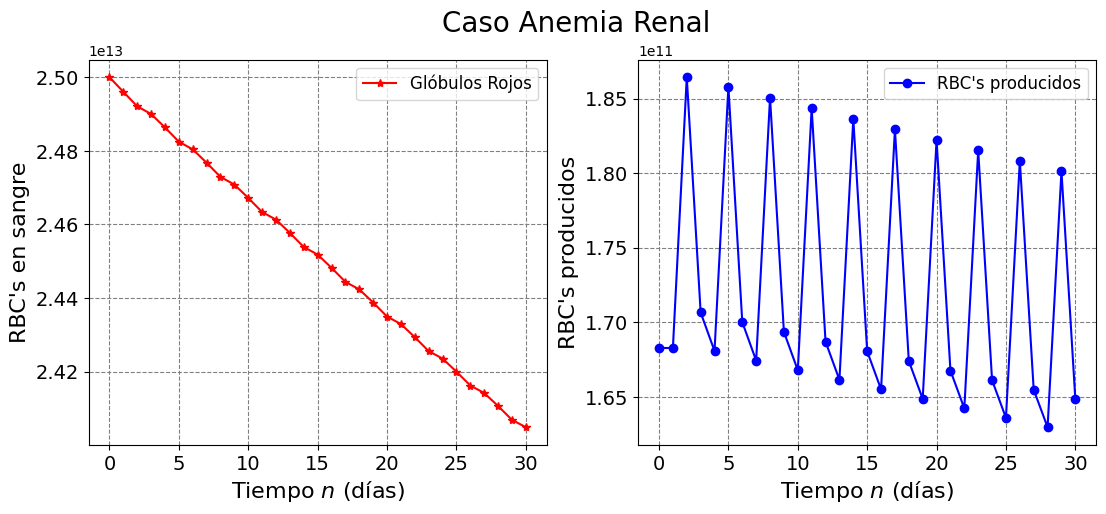
\includegraphics[scale=0.526]{figures/AR11.png}
    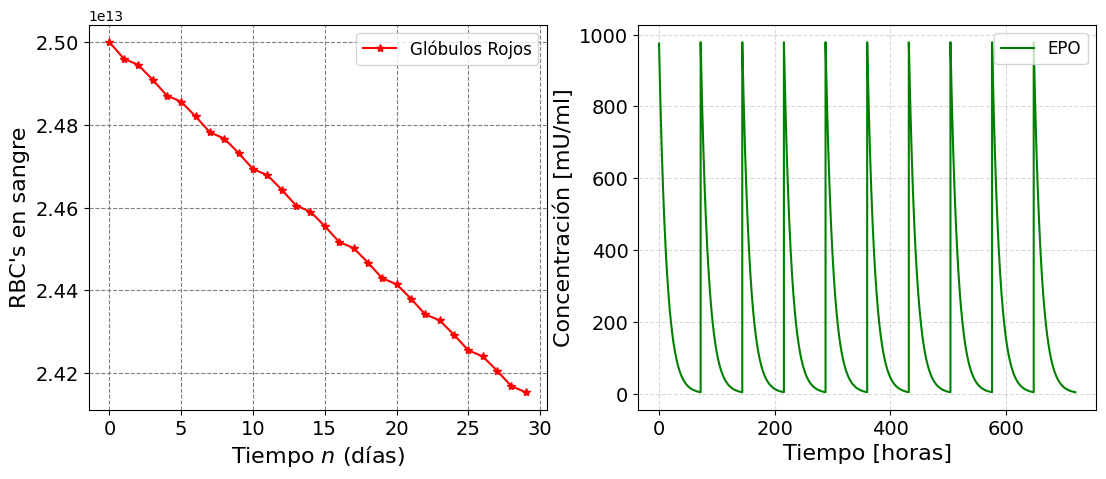
\includegraphics[scale=0.8]{figures/AR12.png}
    \caption{Simulación del modelo para el caso de anemia renal con dosis de EPO de 975 mU/ml. A la izquierda está la gráfica de $R(n)$, a la derecha la de $M(n)$, abajo la de $\delta(t)$.}
    \label{sec:variaciones:fig:Anemia1}
\end{figure}

Como bien se puede ver en la figura \ref{sec:variaciones:fig:Anemia1}, la dosis de EPO administrada no es suficiente para sanar la constante pérdida de glóbulos rojos en el paciente, pues $R(n)$ presenta una disminución en el tiempo, que al infinito se vuelve 0. Sin embargo, la simulación muestra como cada dosis aplicada hace que el cuerpo aumente de una manera significativa su producción de eritrocitos, como se ve en la gráfica para $M(n)$. Es interesante ver como, según la gráfica inferior, el cuerpo consume la dosis administrada a gran velocidad: al final del primer día queda muy poca concentración de la dosis en el cuerpo (el 15$\%$).

Se concluye que la dosis aplicada de 975 mU/ml no es suficiente para que se contrarresten los efectos de la anemia renal del paciente. De esta manera, se debe encontrar un valor de la dosis para que el paciente logre estabilizar su cantidad de eritrocitos.

\subsection{Concentración de Dosis = 4824 mU/ml}\label{subsec:variaciones:anemia:bien}

Para hallar una concentración de dosis que permita lograr que el paciente logre evitar una pérdida constante de sus eritrocitos, se realizaron varias simulaciones. Con una dosis de $\delta_0 = 4824$ [mU/ml] se logra llegar al resultado esperado. El aumento respecto a la dosis teórica presentada de $975$ mU/ml es del 494.7$\%$. 

Para la concentración de 4824 mU/ml de dosis de EPO, se tienen los siguientes valores iniciales y de los parámetros para el modelo \ref{eq:ModeloAnemia}:

\begin{itemize}
    \item $R(0) = 25\times 10^{12};$ (valor inicial de RBC's)
    \item $f=0.00832;$ (fracción de RBC's eliminada cada día)
    \item $M(0) = R(0)\cdot f \cdot \gamma = 145.6\times 10^{9};$ (RBC's producidos por la médula ósea en el día 0)
    \item $\gamma = 0.809;$ (RBC's producidos por cada uno perdido en un paciente anémico) 
    \item $y_s = 208\times 10^{12};$ (RBC's producidos por la médula ósea por un paciente sano)
    \item $\delta_0=4824$ es la concentración de cada dosis [mU/ml];
    \item $k_e=0.077$ (constante de eliminación) [$\textrm{h}^{-1}$];
    \item $t_0=72$ es el tiempo que debe pasar entra cada dosis [h].
\end{itemize}

La figura \ref{sec:variaciones:fig:Anemia2} muestra como, gracias a la nueva dosis, el cuerpo es capaz de lograr una oscilación constante y casi estable (aumenta muy ligeramente cada día), teniendo un valor máximo de RBC's ligeramente superior al original. La función $R(n)$ se vuelve periódica con un máximo de $25.0213\times 10^{12}$ glóbulos rojos, un aumento del $0.085\%$ respecto al valor original, los valles de la gráfica ocurren para valores de $24.96\times 10^{12}$ eritrocitos, una cantidad $0.16\%$ menor respecto al valor normal. La gráfica derecha, que ilustra los valores de $M(n)$, también muestra la oscilación esperada, con un máximo de 269.004$\times 10^{9}$ que representa un aumento del 29.3$\%$ respecto al valor de glóbulos rojos producidos por una persona sana. Para estos picos de $M(n)$, el paciente tiene una concentración de EPO en sangre de 4832.9 mU/ml, que corresponde a un aumento del 439.35$\%$ respecto a la concentración para pacientes sanos, y una del 543.02$\%$ para el paciente anémico. La gráfica inferior muestra nuevamente cómo el cuerpo consume a gran velocidad la droga administrada. 

\begin{figure}[H]
    \centering
    \captionsetup{justification=centering}
    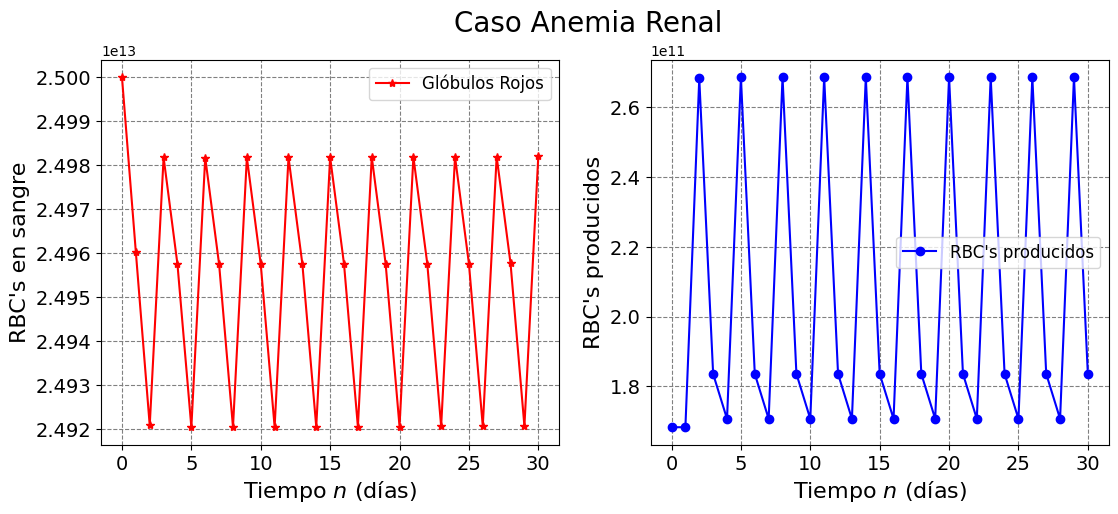
\includegraphics[scale=0.526]{figures/AR21.png}
    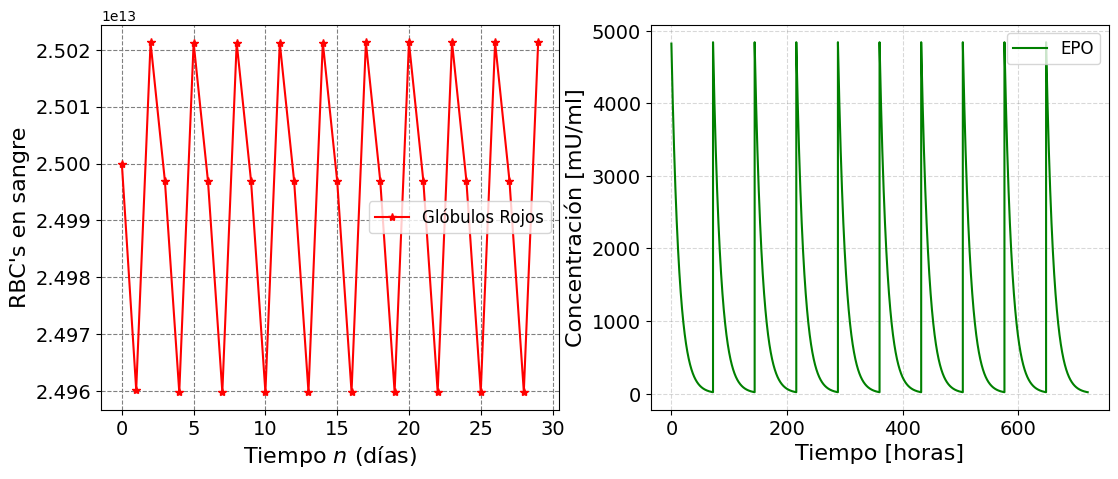
\includegraphics[scale=0.8]{figures/AR22.png}
    \caption{Simulación del modelo para el caso de anemia renal con dosis de EPO de 4824 mU/ml. A la izquierda está la gráfica de $R(n)$, a la derecha la de $M(n)$, abajo la de $\delta(t)$.}
    \label{sec:variaciones:fig:Anemia2}
\end{figure}

Las gráficas muestran que se logran complementar los valles con picos que sobrepasan la concentración normal, lo que permite compensar las deficiencias traídas por la baja cantidad de RBC's. Así, el paciente podrá tener una mejor vida gracias a las dosis del medicamento.

Note ahora que el tamaño de la dosis aplicada depende significativamente del grado de anemia que presenta el paciente. Según el estudio de Panjeta, para los pacientes con anemia renal de tercer grado la concentración media de EPO es de 10.2 mU/ml, por lo que la dosis será mucho menor (según las simulaciones es aproximadamente de 1838 mU/ml).

Las variaciones del modelo presentadas a lo largo del capítulo actual logran evidenciar los resultados esperado según las enfermedades propuestas y sus respectivos tratamientos médicos. En el siguiente capítulo se presentarán las conclusiones de la investigación realizada.